\chapter{Resultat}
Kurz gesagt: Wir konnten fast alle unsere Anforderung erfüllen.

\section{Maturitätsarbeit}
% \includegraphics[height=18cm]{resources/diagrams/use-case}
\begin{enumerate}
    \item \textbf{Zeit} \\
        Geplant war ungefähr eine Lektion pro Woche. Wir haben die geschätzten 100 Stunden (50 Stunden pro Person) um den Faktor vier überschritten. Unser gemessener Zeitaufwand während des aktiven Programmierens
        beträgt über 420 Stunden. Hier sind die Stunden, in denen wir uns in der Schule über das Projekt unterhalten haben, nicht notiert.
    \item \textbf{Begleitperson} \\
        Wir hatten glücklicherweise kein Problem eine Begleitperson zu finden. Martin Hunziker war gerne bereit, unsere Arbeit im Blick zu behalten.
    \item \textbf{Plagiat} \\
        Einige Grafiken sind zwar aus dem Internet, jedoch sind alle nutzungsfrei. Wir haben keinen Code geklaut und verwendet. 
\end{enumerate}

\section{Spiel}
In den folgenden Teilkapiteln wird die Erfüllung der in \autoref{chap:foo} gestellten Anforderungen gruppiert dargestellt. 
\subsection{Notwendig}
    \begin{itemize}
    \item \textbf{Systemanforderungen} \\
        Unser Spiel funktioniert sowohl auf macOS als auch auf Windows. Es läuft zudem mit einer FPS von 300, bis teilweise 500, bei den meisten modernen Rechnern.
    \item \textbf{Benutzeroberfläche} \\
    \begin {itemize}
        \item \textbf{Startseite} \\
            Unsere Startseite hat einen ''Spielen''-Knopf, einen ''Einstellungen''-Knopf, einen ''Credits''-Knopf und einen ''Verlassen''-Knopf. Unsere Tester bewerteten die Startseite
            als intuitiv verständlich. Bedienbar mit der Maus, hatten die Tester keine Probleme sich zurechtzufinden.
            \begin{center}
                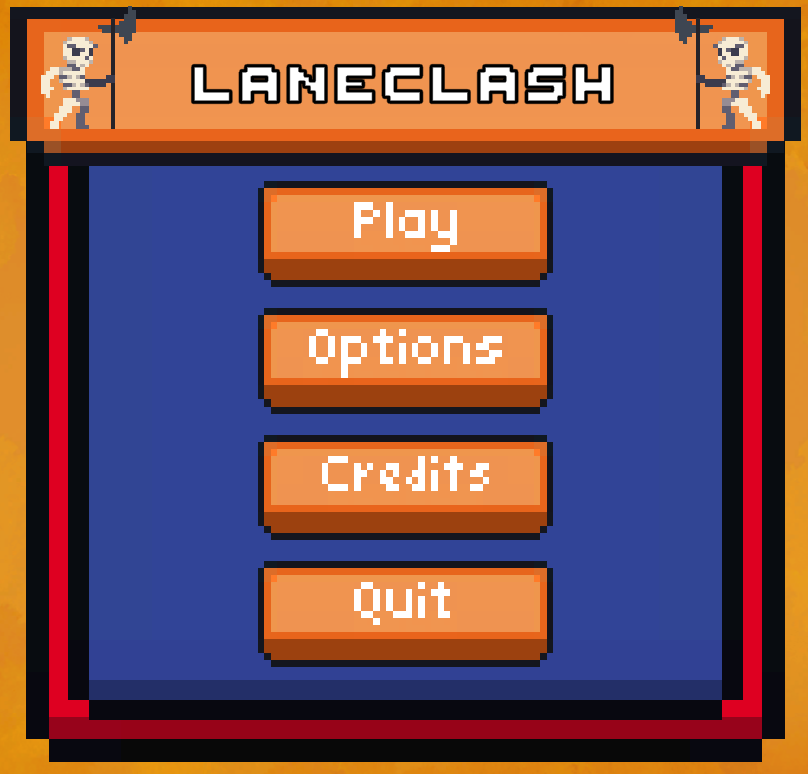
\includegraphics[height=7cm]{resources/laneclash.png}\\
            \end{center}

        \item \textbf{Credits}\\
            Es gibt die Möglichkeit, die Credits vorzeitig zu verlassen. Dies geschieht durch das Drücken des Hausbuttons. Die Tester fanden dies auch sehr intuitiv.
            \begin{center}
                \includegraphics*[width = 7cm]{resources/credits.png}\\
            \end{center}
            
        \item \textbf{Settings}\\
            Man kann hier die Auflösung ändern und auswählen, ob das Spiel als Vollbild dargestellt werden soll. Auch gibt es hier die Möglichkeit, die Musik lauter oder leiser zu stellen
            oder zu muten. Wenn man Einstellungen geändert hat, muss man das Speichern bestätigen. 
            \begin{center}
                \includegraphics*[height=7cm]{resources/setting.png}\\
            \end{center}
            Nach Bestätigung der Änderung der Grafikoptionen, werden die Änderungen angewendet und man hat zehn Sekunden Zeit erneut zu bestätigen. Sonst werden die Änderungen zurückgesetzt.
            Dies wurde implementiert, um eventuellen Problemen vorzubeugen. 
            \begin{center}
                \includegraphics*[height=3cm]{resources/resolution.png}\\
            \end{center}
            
        \item \textbf{Server Management}\\
            Nach Bedienung des ''Start''-Knopfs gibt es die Möglichkeit, einen Server zu hosten oder einer bereits existierenden Lobby als Client beizutreten. Ausserdem kann man
            automatisch nach bereits existierenden Servern suchen.
            \begin{center}
                \includegraphics*[height = 3cm]{resources/server.png}\\
            \end{center}
            Den Server kann man mit einem Linksklick auswählen.
            \begin{center}
                \includegraphics*[width=6cm]{resources/discovered.png}\\
            \end{center}
            
        \item \textbf{Lobby Management}\\
            Player (1) ist dabei immer der Host, und Player (2) immer der Client. Das eigentliche Spiel beginnt erst, sobald beide Spieler bereit, also ''ready'', sind. 
            Der Status ''ready'' wird dabei immer aktualisiert dargestellt. Der Host hat ausserdem die Möglichkeit, den Spieler (2) aus der Lobby zu entfernen. 
            \begin{center}
                \includegraphics*[width = 5cm]{resources/lobby.png} \includegraphics*[width=5cm]{resources/lobbyc.png}\\ 
            \end{center}
            
        \item \textbf{InGame-UI}\\
            Der Host hat die Möglichkeit, das Spiel zu beenden. Er kann auch direkt aufhören zu hosten. 
            Auch der Client hat durchgehend die Möglichkeit, den Server zu verlassen.
            \begin{center}
                \includegraphics*[height=2cm]{resources/returnlobby.png} \includegraphics*[height=2cm]{resources/stopclient.png}\\
            \end{center}
            Im Pausenmenu kann man ausserdem leicht die Musiklautstärke und die Stärke des Schneefalls ändern. Dieses Menu kann mit ESC geöffnet und geschlossen werden.
            \begin{center}
                \includegraphics*[height=2cm]{resources/pause.png}\\
            \end{center}
            
            


    \end {itemize}

    \item \textbf{Lokaler Multiplayer} \\
        Das Spiel kann im lokalen Netz gespielt werden. Zum Testen kann man das Spiel auch zweimal parallel auf demselben Gerät laufen lassen. Als Protokoll haben wir TCP gewählt.
        Folgende vier Punkte waren entscheidend für die Wahl von TCP gegenüber UDP:
        \begin{itemize}
            \item \textbf{Zuverlässigkeit}\\
                Es gibt keine Probleme mit verloren gegangenen Paketen. Ging ein Paket verloren, sendet TCP es einfach erneut. Entweder werden alle Daten erfolgreich übermittelt,
                oder es folgt eine Errormeldung.
            \item \textbf{Sequenziert}\\
                TCP stellt sicher, dass jede Nachricht in der gleichen Reihenfolge eintrifft, in der sie gesendet wurde. Wenn man ''a'' vor ''b'' sendet, erhält man auf der
                anderen Seite garantiert auch zuerst ''a'' und dann ''b''.
            \item \textbf{Verbindungsorientiert}\\
                TCP hat sich auf das Konzept einer Verbindung spezialisiert. Eine Verbindung bleibt so lange geöffnet, bis entweder der Client oder der Server sich dazu entscheiden, sie zu schliessen.
                Anschliessend werden sowohl Client als auch Host benachrichtigt, dass die Verbindung beendet wurde.
            \item \textbf{Überlastungskontrolle} \\
                Wenn ein Server überlastet wird, drosselt TCP selbstständig die Daten, um einen Zusammenbruch durch Überlastung zu verhindern.


        \end{itemize}
    \item \textbf{Einstellungen} \\
        Auflösung, Vollbild, Lautstärke und Stärke des Schneefalls können eingestellt werden.
    \item \textbf{Kamera} \\
        Die Kamera ist beweglich und das ganze Schlachtfeld ist sichtbar. Mit den Pfeiltasten kann man die Kamera frei bewegen und hinein- bzw. hinauszoomen.
    \item \textbf{Truppen} \\
        IMPORTANT\\
        IMPORTANT\\
        IMPORTANT\\
        IMPORTANT\\
        IMPORTANT\\
        IMPORTANT\\
        IMPORTANT\\
        IMPORTANT\\
        IMPORTANT\\
        IMPORTANT\\
        IMPORTANT\\
        IMPORTANT\\
        IMPORTANT\\
        IMPORTANT\\
        IMPORTANT\\
        IMPORTANT\\
        IMPORTANT\\
    \item \textbf{Spielende} \\
        Um zu gewinnen, muss eine eigene Truppe die Portale des Gegners durchschreiten. Dies verhindern zuerst sogenannte Helden. Sterben jene Helden, erledigt ihr Racheeffekt alle
        Truppen, die sich auf jener Linie des Helden befanden.
    \item \textbf{Lanes} \\
        Unser Spiel hat vier sogenannte Linien (''Lanes''). Diese unterschiedlichen Linien wurden in der Tiefe nach hinten verschoben. Der Spieler hat die Auswahl, in welcher Reihe er seine Truppen auf den Gegner zuschicken will.
    \item \textbf{Synchronisation} \\
        Unser Spiel synchronisiert alle Daten in Echtzeit. Dadurch sehen alle Spieler immer dasselbe. Wird der Client aus einem unbekannten Grund disconnected, kann er versuchen,
        sich erneut zu verbinden, und der Server wird dann direkt alle Daten synchronisieren. Auch hier hilft uns das gewählte Protokoll TCP. Geht ein Paket verloren, wird es automatisch
        erneut gesendet. Dies hilft uns dabei, die Synchronisation zu jeder Zeit aufrechtzuerhalten.
    \item \textbf{Crossplay}
        Es ist möglich, sich mit einem Windows Rechner und einem macOS Rechner zu verbinden. Allerdings muss dem Spiel dazu die Kommunikation durch die Firewall teilweise erlaubt sein.
        Bei einer eher aggressiveren Firewall wird zudem teilweise der Server-Broadcast geblockt. Dies hätte zur Folge, dass man die Server nicht automatisch finden kann. 
        Verbinden kann mich sich allerdings trotzdem noch.   
\end{itemize}

\subsection{Anvisiert}
\begin{itemize}
    \item \textbf{Helden} \\
        Beide Spieler haben bei unserer aktuellen Version den gleichen Heldentyp. Dies ist ein magischer Turm. Er hat keine Angriffsmöglichkeiten. Allerdings kann er sich passiv heilen und so als eine
        temporäre Grenze zwischen den gegnerischen Truppen und den eigenen Portalen agieren. Die eigenen Truppen werden durch diese Portale hinter den Helden gespawned.
    \item \textbf{Design} \\
        Wir haben uns für ein 2.5d Design entschieden. Der Vorteil ist, dass wir 2d Grafiken benutzen können. Die Sprites werden dabei um 45 Grad gedreht. Auch 
        die Kamera schaut in einem 45 Grad Winkel auf das Geschehen. Dadurch ergibt sich die Illusion einer Perspektive, in der man von der Seite auf das Geschehen schaut. 
        \begin{center}
            \includegraphics*[height=5cm]{resources/25d.png} \includegraphics*[height=5cm]{resources/25dtwo.png}\\
        \end{center}
        
    \item \textbf{Effekte}
    \begin{itemize}
        \item \textbf{Gift:}
        Zeitlich limitierter und sich wiederholender Schadenseffekt.
        Eine visuelle Markierung ist vorhanden und der Gifteffekt kumuliert sich nicht (hier: Pilz-Truppe).
        \item \textbf{Rache:}
            Truppen mit Rache haben einen Effekt nach ihrem Tod. Sie können zum Beispiel eine Truppe beschwören oder Schaden verursachen (hier: Helden mit Feuer).
    \end{itemize}
\end{itemize}

\subsection{Möglich}
\begin{itemize}
    \item \textbf{Monetarisierung} \\
    \begin{enumerate}
        \item \textbf{Kostenpflichtiges Spiel}
        \begin{itemize}
            \item Wir haben eventuell vor, unser Spiel nach Vollendung der Entwicklungsphase zu veröffentlichen. Allerdings wird der Preis auf keinen Fall hoch sein.
        \end{itemize}
    \end{enumerate}
    \item \textbf{Design} \\
        Wir werden auch in Zukunft das Design noch verbessern. 
    \item \textbf{Truppen}
        Weitere Truppen können jederzeit erstellt werden. Hier ist kein Limit gesetzt: Leben, Schaden, Darstellung, Effekt und vieles mehr kann angepasst werden. 
        Wir haben alle Programme mit dem Hintergedanken geschrieben, dass es jederzeit ohne grössere Anpassungen möglich ist, neue Truppen hinzuzufügen.
    
\end{itemize}

\subsection{Fürs Erste verworfen}
\begin{itemize}
    \item \textbf{Online Multiplayer} \\
        Um sich mit Rechnern ausserhalb des eigenen Netzwerkes verbinden zu können, müssten wir das ganze Multiplayer-System unseres Spieles anpassen, was einen kompletten \gls{Recode} zur Folge hätte. 
        Ausserdem, würde sich die Frage nach der Finanzierung stellen, falls wir einen externen Server kaufen / mieten würden. 
    \item \textbf{Shop} \\
        Ein Shop ohne Anti-Cheat und/oder Server ist die perfekte Angriffsfläche für Cheater und ist somit für uns nicht sinnvoll. Wir müssten dann ausserdem ein Ranking-System
        hinzufügen, damit wir die Spieler belohnen können.
    \item \textbf{Kampagne} \\
        Unser Spiel ist vor allem auf den Multiplayer ausgelegt. Eine Kampagne setzt ausserdem voraus, dass man einen offline Gegner (''Bot'') hat. Wir haben uns bereits 
        früh gegen eine Kampagne entschieden, da diese in diesem Stadium leider unsere Kapazität überschreitet.
    \item \textbf{Anti-Cheat} \\
        Wir haben keine Erfahrung in diesem Bereich und es ist ein extrem komplexes Thema. Allerdings hat der Host sozusagen über fast alles die Macht, der Client kann also fast
        gar nichts kaputtmachen. Wir hoffen ausserdem auf die Ehrlichkeit der Menschen, die unser Spiel spielen.
    \item \textbf{Errungenschaften} \\
        Belohnungen zu erhalten ist immer toll. Wir haben zwei Arten von möglichen Belohnungen diskutiert und verworfen: eine Währung und / oder Pokale.
        Für die Währung bräuchten wir allerdings auch einen Shop. Wir müssten ausserdem neue Gegenstände hinzufügen,
        die man zuerst erspielen muss. Für die Pokale bräuchten wir ein Ranking-System.
    \item \textbf{Bot} \\
        Ein guter Bot passt sich der Spielweise des Gegners an. Einen so guten Bot zu programmieren ist eine Herausforderung für sich. Wir hatten die Idee,
        dass der Bot immer zufällige Truppen zu zufälligen Zeiten spielt. Allerdings würde dies auch eine Menge Balancing benötigen, wofür wir im Moment leider zu wenig
        Zeit haben.
    \item \textbf{Helden} \\
        Wir hatten als Ziel, mehrere verschiedene Helden zu gestalten und zu programmieren. Allerdings stellte sich relativ früh heraus, dass wir die nötigen Ressourcen
        lieber an einer anderen Stelle investieren. Wir haben nun einen einzigen Helden, allerdings würde sich das Ausbauen der Helden nach der Abgabe als spannend gestalten.
        Die Grundlage für den Ausbau ist bereits vorhanden.
    \item \textbf{Ingame-Chatfenster}\\
        Wir hatten eine funktionierende Version erstellt und implementiert. Allerdings stellte sich dies als überflüssig heraus, da man normalerweise neben der Person sitzt,
        mit der man im Moment spielt.
    \item \textbf{Mehrsprachig} \\
        Das Spiel ist im Moment nur in Englisch verfügbar. Eventuell werden wir dies nach der Abgabe der schriftlichen Arbeit noch anpassen.
    \item \textbf{Effekte}
    \begin{itemize}
        \item \textbf{Wiederbelebung:}
            Die Möglichkeit einer Wiederbelebung würde sich nur für spezielle Truppen anbieten. Er würde den Spieler wahrscheinlich ein Vielfaches davon kosten,
            als wenn er neue Truppen losschicken würde. 
        \item \textbf{Rüstung:}
            Uns schien dies nicht nötig zu sein. Dies würde sich erst lohnen, sobald wir mehr Truppen, Effekte oder anderes hinzugefügt hätten.
        \item \textbf{Aura:}
            Das Prinzip einer Aura klingt faszinierend. Allerdings hätte dies sehr wahrscheinlich einen Recode des Damage-Systems zur Folge und würde unsere Ressourcen sprengen.
    \end{itemize}
    \item \textbf{Tutorial} \\
        Da wir bei der Entwicklung einen Schwerpunkt auf die intuitive Bedienbarkeit gelegt haben, konnten wir auf ein Tutorial und den damit verbundenen immensen Zeitaufwand verzichten.
    \item \textbf{Monetarisierung} \\
    Ohne Anti-Cheat leider vollkommen nutzlos.
    \begin{enumerate}
        \item \textbf{Kaufbare Gegenstände}
        \begin{itemize}
            \item Neben Schummelmöglichkeiten stellt sich hier ausserdem die Gefahr eines möglichen Pay-to-Win.
        \end{itemize}
        \item \textbf{Skins}
        \begin{itemize}
            \item Der Spieler bräuchte ein Inventar, das mit einem Server kontrolliert und synchronisiert wird. 
        \end{itemize}
    \end{enumerate}
    \item \textbf{Zauber} \\
        Wir hatten bereits zu einem frühen Zeitpunkt eine funktionierende Testversion. Der Zauber wurde dem Spieler durch Karte verteilt. \\
        Im Laufe der Zeit haben wir das Damage-System allerdings so umgeändert, dass der Prototyp schon fast nutzlos war. Ein kompletter Recode des Prototypen wäre nötig.
    \begin{itemize}
        \item \textbf{Dornen:}
            Nachdem wir den Zauber ''Gift'' hinzugefügt hatten, erschien und das zusätzliche Hinzufügen der Dornen überflüssig.
    \end{itemize}
    \item \textbf{Deck} \\
        Die Möglichkeit, sich ein eigenes Deck zusammenzustellen, aus dem man dann die Karten zieht, wurde leider aus Zeitgründen fürs Erste verworfen. Allerdings können wir
        fast schon garantieren, dass wir dies bis zu unserer Präsentation noch hinzufügen werden.     
\end{itemize}